\documentclass[12pt]{mypackage}

% sans serif font:
%\usepackage{cmbright}
%\usepackage{sfmath}
%\usepackage{bbold} %better blackboard bold

%serif font + different blackboard bold for serif font
\usepackage{newpxtext,eulerpx}
\renewcommand*{\mathbb}[1]{\varmathbb{#1}}

\pagestyle{fancy} %better headers
\fancyhf{}
\rhead{Avinash Iyer}
\lhead{Physics 310, Assignment 1}

\setcounter{secnumdepth}{0}

\begin{document}
\section{Chapter 2 Problems}%
\subsection{2.3}%
\subsubsection{Cylindrical Coordinates}%
Starting with our expression of $\mathbf{r}$, we have
\begin{align*}
  \mathbf{r} &= \rho \cos\phi \hat{i} + \rho \sin\phi\hat{j} + z\hat{k}\\
  d\mathbf{r} &= \pd{\mathbf{r}}{\rho}d\rho + \pd{\mathbf{r}}{\phi}d\phi + \pd{\mathbf{r}}{z}dz.
  \intertext{Calculating each partial derivative,}
  \pd{\mathbf{r}}{\rho} &= \cos\phi \hat{i} + \sin\phi\hat{j}\\
  \hat{\rho} &= \frac{\pd{\mathbf{r}}{\rho}}{\left\Vert \pd{\mathbf{r}}{\rho} \right\Vert}\\
             &= \cos\phi\hat{i} + \sin\phi\hat{j},\\
  \pd{r}{\phi} &= \rho \left(-\sin\phi \hat{i} + \cos\phi\hat{j}\right)\\
  \hat{\phi} &= \frac{\pd{\mathbf{r}}{\phi}}{\left\Vert \pd{\mathbf{r}}{\phi} \right\Vert}\\
             &= -\sin\phi\hat{i} + \cos\phi\hat{j}
             \intertext{implying}
  \pd{\mathbf{r}}{\phi} &= \rho\hat{\phi},
  \intertext{and finally, we have}
  \pd{\mathbf{r}}{z} &= \hat{k}.
  \intertext{The above calculations yield}
  d\mathbf{r} &= \left(d\rho\right) \hat{\rho} + \left(\rho\,d\phi\right)\hat{\phi} + \left(dz\right)\hat{k}.
\end{align*}
\subsubsection{Spherical Coordinates}%
  Starting with our expression of $\mathbf{x}$\footnote{I am using $\mathbf{x}$ instead of $\mathbf{r}$ because $r$ is already used in the expression of the spherical coordinates.}
\begin{align*}
  \mathbf{x} &= r\sin\phi\sin\theta\hat{i} + r\cos\phi\sin\theta\hat{j} + r\cos\theta\hat{k}\\
  d\mathbf{x} &= \pd{\mathbf{x}}{r}dr + \pd{\mathbf{x}}{\phi}d\phi + \pd{\mathbf{x}}{\theta}d\theta,
  \intertext{Evaluating each partial derivative, we have}
  \pd{\mathbf{x}}{r} &= \sin\phi\sin\theta\hat{i} + \cos\phi\sin\theta\hat{j} + \cos\theta\hat{k}\\
  \hat{r} &= \frac{\pd{\mathbf{x}}{r}}{\left\Vert \pd{\mathbf{x}}{r} \right\Vert}\\
  &= \sin\phi\sin\theta\hat{i} + \cos\phi\sin\theta\hat{j} + \cos\theta\hat{k},\\
  \pd{\mathbf{x}}{\phi} &= -r\sin\phi\sin\theta\hat{i} + r\cos\phi\sin\theta\hat{j}\\
  \hat{\phi} &= \frac{\pd{\mathbf{x}}{\phi}}{\left\Vert \pd{\mathbf{x}}{\phi} \right\Vert}\\
             &= -\sin\phi\sin\theta\hat{i} + \cos\phi\sin\theta\hat{j}
             \intertext{implying}
  \pd{\mathbf{x}}{\phi} &= r\sin\theta \hat\phi,
  \intertext{and finally, we have}
  \pd{\mathbf{x}}{\theta} &= r\cos\phi\cos\theta\hat{i} + r\sin\phi\cos\theta\hat{j} - r\sin\theta\hat{k}\\
  \hat\theta &= \frac{\pd{\mathbf{x}}{\theta}}{\left\Vert \pd{\mathbf{x}}{\theta} \right\Vert}\\
             &= \cos\phi\cos\theta\hat{i} + \sin\phi\cos\theta\hat{j} - \sin\theta\hat{k},
             \intertext{implying}
  \pd{\mathbf{x}}{\theta} &= r\hat\theta.
  \intertext{The above calculations yield}
  d\mathbf{x} &= \left(dr\right)\hat{r} + \left(r\sin\theta d\phi\right)\hat{\phi} + \left(rd\theta\right)d\theta.
\end{align*}
\subsection{2.8}%
Let
\begin{align*}
  \vec{a} &= r_a\cos\phi_a\sin\theta_a \hat{i} + r_a\sin\phi_a\sin\theta_a\hat{j} + r_a\cos\theta_a\hat{k}\\
  \vec{b} &= r_b\cos\phi_b\sin\theta_b \hat{i} + r_b\sin\phi_b\sin\theta_b\hat{j} + r_b\cos\theta_b\hat{k}.
\end{align*}
Then,
\begin{align*}
  \cos\gamma &= \frac{\vec{a}\cdot\vec{b}}{\left\Vert \vec{a} \right\Vert\left\Vert \vec{b} \right\Vert}\\
             &= \frac{1}{r_ar_b} \left(r_ar_b\left(\sin\theta_a\sin\theta_b\left(\cos\phi_a\cos\phi_b + \sin\phi_a\sin\phi_b\right) + \cos\theta_a\cos\theta_b\right)\right)\\
             &= \cos\theta_a\cos\theta_b + \sin\theta_a\sin\theta_b\cos\left(\phi_a-\phi_b\right).
\end{align*}
\subsection{2.9}%
\begin{align*}
  \diff{\vec{v}}{t} &= \diff{}{t}\left(\dot{\rho}\hat\rho\right) + \diff{}{t}\left(\rho\dot\phi\hat\phi\right)\\
                    &= \hat{\rho}\ddot{\rho} + \dot\rho\frac{d\hat\rho}{dt} + \dot\rho\dot\phi\hat{\phi} + \rho\ddot\phi\hat\phi + \rho\dot\phi\frac{d\hat{\phi}}{dt}\\
                    &= \hat\rho\ddot\rho + \dot\rho\dot{\phi}\hat\phi + \rho\ddot\phi\hat\phi + \dot\rho\dot\phi\hat\phi + \left(\pd{\hat\phi}{\rho}\frac{d\rho}{dt} + \pd{\hat\phi}{\phi}\frac{d\phi}{dt}\right)\\
                    &= \left(\ddot\rho - \rho\dot\phi^2\right) \hat{\rho} + \left(\rho\ddot\phi + 2\dot\rho\dot\phi\right)\hat{\phi}.
\end{align*}
\subsection{2.12}%
\begin{enumerate}[(a)]
  \item \hfill
    \begin{enumerate}[(i)]
      \item $d\mathbf{a} = \rho\:d\phi dz$
      \item $d\mathbf{a} = d\rho dz$
      \item $d \mathbf{a} = \rho\:d\rho d\phi$
    \end{enumerate}
  \item \hfill
    \begin{enumerate}[(i)]
      \item $d\mathbf{a} = r^2\sin \theta\:d\theta d\phi$
      \item $d\mathbf{a} = r \sin \theta\:dr d\phi$
      \item $d\mathbf{a} = r\:drd\theta$
    \end{enumerate}
\end{enumerate}
\subsection{2.14}%
\begin{enumerate}[(a)]
  \item 
    \begin{align*}
      d\Phi &= \mathbf{E}\cdot \hat{n}\: dA\\
            &= \norm{\mathbf{E}}\norm{\hat{n}}\cos\theta dA\\
            &= \frac{q}{4\pi\epsilon_0 r^2}\cos\theta dA.
    \end{align*}
    \begin{center}
      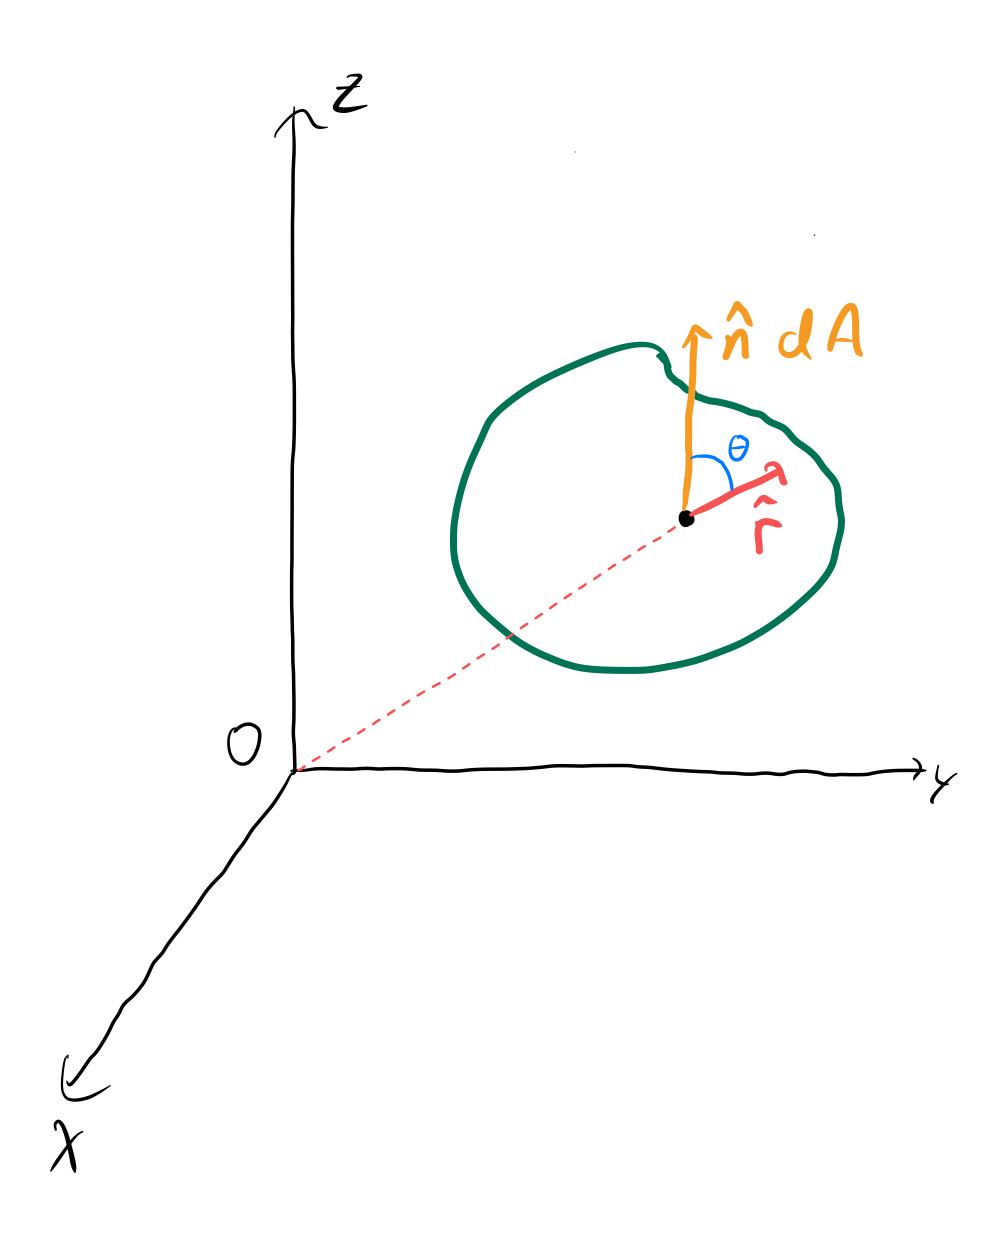
\includegraphics[width=8cm]{images/p_1a_1_2-14a}
    \end{center}
    \item\hfill
      \begin{center}
        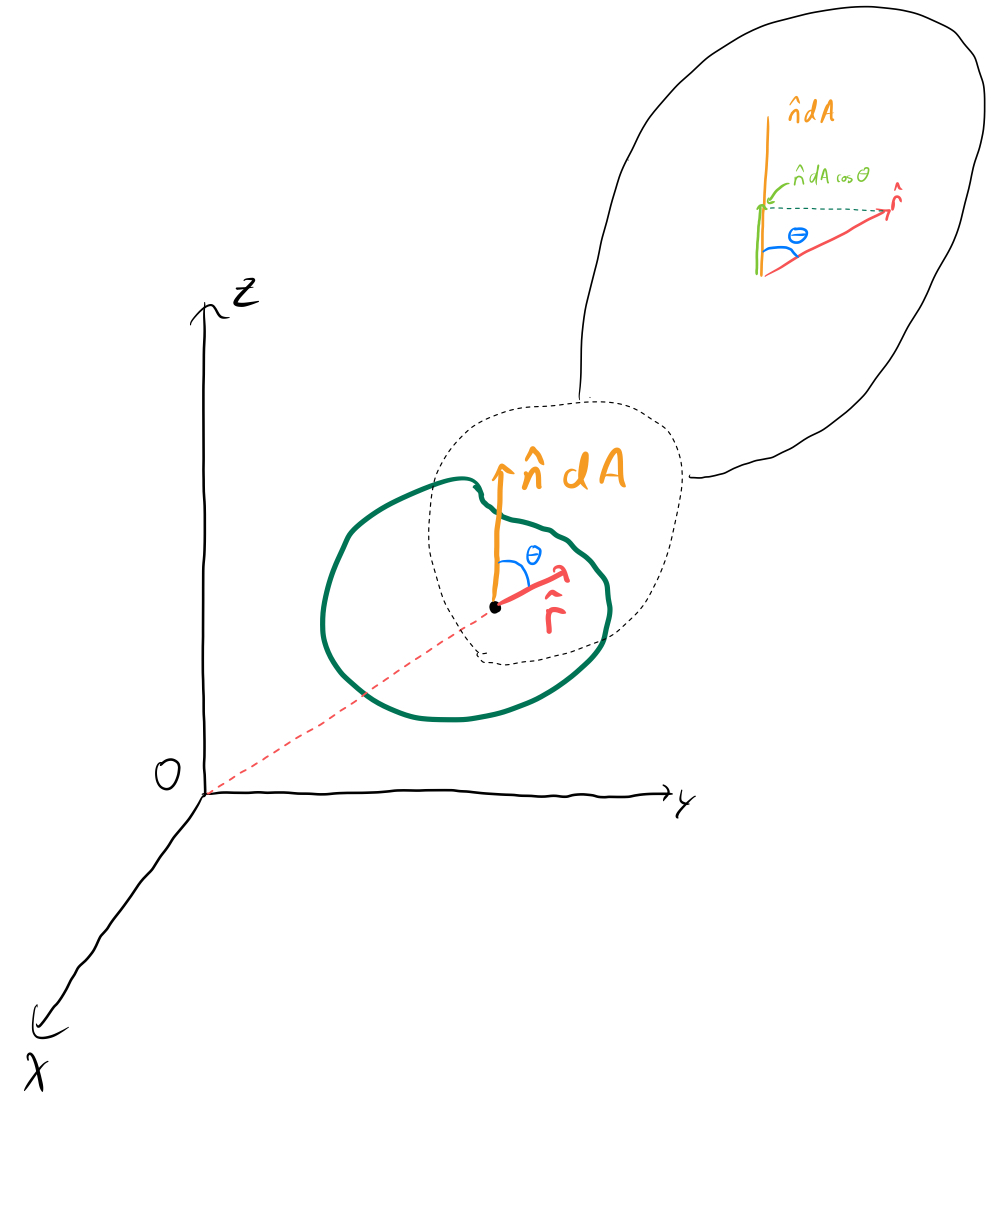
\includegraphics[width=8cm]{images/p_1a_1_2-14b}
      \end{center}
    \item 
      \begin{align*}
        \oiint_{S}^{} \:d\Phi &= \oiint_{S}^{} \frac{q}{4\pi \epsilon_0 r^2}\:d\mathbf{a}\\
                              &= \int_{0}^{2\pi}\int_{0}^{\pi}\frac{q}{4\pi \epsilon_0 r^2}r^2\sin\theta\:d\theta d\phi\\
                              &= \left(2\pi\right)\left(\frac{q}{4\pi \epsilon_0}\right)\left(-\cos\theta\bigr\vert_{0}^{\pi}\right)\\
                              &= \frac{q}{\epsilon_0}.
      \end{align*}
\end{enumerate}
\section{Chapter 3 Problems}%
For all problems involving $\arg z$ (or equivalents), I will be using the principle branch, $\arg z \in (-\pi,\pi]$.
\subsection{3.5}%
\begin{enumerate}[(a)]
  \item
    \begin{align*}
      \sqrt{3} + i &= 2e^{i\frac{\pi}{3}}\\
      -\sqrt{3} + i &= 2e^{i\frac{2\pi}{3}}
    \end{align*}
  \item 
    \begin{align*}
      \sqrt{2i} &= \sqrt{2}e^{i \frac{\pi}{4}}\\
      \sqrt{2 + 2\sqrt{3}i} &= 2e^{i \frac{\pi}{6}}
    \end{align*}
\end{enumerate}
\section{3.6}%
\begin{enumerate}[(a)]
  \item Real:
    \begin{align*}
      \left(-1\right)^{1/i} &= \left(e^{i\pi}\right)^{-i}\\
                            &= e^{\pi}.
    \end{align*}
  \item Real:
    \begin{align*}
      \left(\frac{z}{z^{\ast}}\right)^{i} &= \left(e^{2i\arg z}\right)^{i}\\
                                          &= e^{-2\arg z}.
    \end{align*}
  \item Imaginary:
    \begin{align*}
      \left(z_1z_2^{\ast} - z_1^{\ast}z_2\right)^{\ast}&= z_1^{\ast}z_2 - z_1z_2^{\ast}\\
                                                       &= -\left(z_1z_2^{\ast} - z_1^{\ast}z_2\right).
    \end{align*}
  \item Complex: 
    \begin{align*}
      \sum_{n=0}^{N}e^{in\theta} &= \frac{1 - e^{iN\theta}}{1 - e^{i\theta}}.
    \end{align*}
  \item Real: for each $a\in \set{1,2,\dots,N}$, $e^{ia\theta} + e^{-ia\theta} \in \R$.
\end{enumerate}
\section{3.9}%
\begin{enumerate}[(a)]
  \item
    \begin{align*}
      \cos\left(a+b\right) + \cos\left(a-b\right) &= \frac{1}{2}\left(e^{i\left(a+b\right)} + e^{-i\left(a+b\right)}\right) + \frac{1}{2}\left(e^{i\left(a-b\right)} + e^{-i\left(a-b\right)}\right)\\
                                                  &= \frac{1}{2}\left(e^{ia}\left(e^{ib} +e^{-ib}\right) + e^{-ia}\left(e^{ib} + e^{-ib}\right)\right)\\
                                                  &= \frac{1}{2}\left(e^{ia} + e^{-ia}\right)\left(e^{ib} + e^{-ib}\right)\\
                                                  &= 2\cos a \cos b.
    \end{align*}
  \item 
    \begin{align*}
      \sin\left(a+b\right) + \sin\left(a-b\right) &= \frac{1}{2i}\left(e^{i\left(a + b\right)} - e^{-i\left(a+b\right)}\right) + \frac{1}{2}\left(e^{i\left(a-b\right)} - e^{-i\left(a-b\right)}\right)\\
                                                  &= \frac{1}{2i}\left(e^{ia}\left(e^{ib} + e^{-ib}\right) - e^{-ia}\left(e^{ib} + e^{-ib}\right)\right)\\
                                                  &= \frac{1}{2i}\left(e^{ia} - e^{-ia}\right)\left(e^{ib} + e^{-ib}\right)\\
                                                  &= 2\sin a \cos b.
    \end{align*}
\end{enumerate}
\section{3.10}%
\begin{enumerate}[(a)]
  \item 
    \begin{align*}
      e^{i\alpha} + e^{i\beta} &= e^{i\left(\frac{\alpha + \beta}{2} + \frac{\alpha - \beta}{2}\right)} + e^{i\left(\frac{\alpha + \beta}{2} - \frac{\alpha - \beta}{2}\right)}\\
                               &= e^{i\frac{\alpha + \beta}{2}}\left(e^{i\frac{\alpha - \beta}{2}} + e^{-i\frac{\alpha - \beta}{2}}\right)\\
                               &= 2\cos\left(\frac{\alpha - \beta}{2}\right)e^{i\frac{\alpha + \beta}{2}}.
    \end{align*}
  \item 
    \begin{align*}
      e^{i\alpha} - e^{i\beta} &= e^{i\left(\frac{\alpha + \beta}{2} + \frac{\alpha - \beta}{2}\right)} - e^{i\left(\frac{\alpha + \beta}{2} - \frac{\alpha - \beta}{2}\right)}\\
                               &=  e^{i\frac{\alpha + \beta}{2}}\left(e^{i\frac{\alpha - \beta}{2}} - e^{-i\frac{\alpha - \beta}{2}}\right)\\
                               &= 2i\sin\left(\frac{\alpha - \beta}{2}\right)e^{i\frac{\alpha + \beta}{2}}
    \end{align*}
\end{enumerate}
\section{3.12}%
\begin{align*}
  \frac{1}{2i}\ln \left(\frac{a + ib}{ a - ib }\right) &= \frac{1}{2i}\left(\ln \left(a + ib\right) - \ln \left(a - ib\right)\right)\\
                                                       &= \frac{1}{2i}\left(\ln |a + ib| + i\arctan\left(\frac{b}{a}\right) - \left(\ln|a + ib| + i\arctan\left(-\frac{b}{a}\right)\right)\right)\\
                                                       &= \arctan\left(\frac{b}{a}\right).
\end{align*}
\section{3.13}%
\begin{align*}
  \diff{^n}{t^n}\left(e^{at}\sin bt\right) &= \frac{1}{2i}\diff{^n}{t^n}\left(e^{\left(a + ib\right)t} - e^{\left(a - ib\right)t}\right)\\
                                           &= \frac{1}{2i}\left((a + ib)^{n}e^{\left(a + ib\right)t} - (a - ib)^{n}e^{\left(a - ib\right)t}\right)\\
                                           &= \frac{1}{2i}e^{at}\left(\left(\left(a^2 + b^2\right)^{n/2}e^{in\arctan\left(\frac{b}{a}\right)}\right)e^{ibt} - \left(\left(a^2 + b^2\right)^{n/2}e^{-in\arctan\left(\frac{b}{a}\right)}\right)e^{-ibt}\right)\\
                                           &= e^{at}\frac{1}{2i}\left(a^2 + b^2\right)^{n/2}\left(e^{i\left(b + n\arctan\left(\frac{b}{a}\right)\right)t} - e^{i\left(b + n\arctan\left(\frac{b}{a}\right)\right)}\right)\\
                                           &= e^{at}\left(a^2 + b^2\right)^{n/2}\sin\left(bt + n\arctan\left(\frac{b}{a}\right)\right)
\end{align*}
\section{3.20}%
Showing the equivalence between $C_1\cos kx + C_2\sin kx$ and $A\cos \left(kx + \alpha\right)$ and $B \sin \left(kx + \beta\right)$, we have
\begin{align*}
  A\cos\left(kx + \alpha\right) &= A\cos kx\cos\alpha - A\sin kx \sin\alpha\\
  B\sin\left(kx + \beta\right) &= B\cos kx \sin\beta + B \sin kx \cos\beta
  \intertext{meaning (assuming $\alpha,\beta \neq \pi n,\pi/2 + \pi n$)}
  A &= \frac{C_1}{\cos\alpha}\\
    &= -\frac{C_2}{\sin\alpha}\\
  B &= \frac{C_1}{\sin \beta}\\
    &= \frac{C_2}{\cos\beta}.
\end{align*}
Now, we show the equivalence between $C_1\cos kx + C_2\sin kx$ and $D_1e^{ikx} + D_2e^{-ikx}$.
\begin{align*}
  D_1e^{ikx} + D_2e^{-ikx} &= \frac{D_1 + D_2}{2}\left(e^{ikx} + e^{-ikx}\right) + \frac{D_1 + D_2}{2}\left(e^{ikx} - e^{-ikx}\right)\\
                           &= \left(D_1 + D_2\right)\cos kx + i\left(D_1 - D_2\right)\sin kx.
  \intertext{meaning}
  C_1 &= D_1 + D_2\\
  C_2 &= i\left(D_1 - D_2\right).
\end{align*}
Finally, we show the equivalence between $\re\left(Fe^{ikx}\right)$ and $C_1\cos kx + C_2\sin kx$.
\begin{align*}
  \re \left(\left(a + ib\right)e^{ikx}\right) &= \re \left(a\cos kx + ia\sin kx + ib \cos kx - b \sin kx\right)\\
                                              &= a\cos kx - b \sin kx,
                                              \intertext{meaning}
  C_1 &= a\\
  C_2 &= -b.
\end{align*}
\end{document}
